\newpage
\section{Cluttered Pick Test}

\subsection{Purpose and Focus of the Test}
The purpose of the \iaterm{Cluttered Pick Test}{CPT} is to evaluate the perception
and manipulation of the robots in a cluttered scenario. The scenario is motivated by
the fact that most of the objects in the factory or labs are always lying in a clutter.


\subsection{Scenario Environment}
The arena used for this test contains basically all elements as for the Basic
Manipulation Test. Two service areas with a height of 10cm are involved in the test,
most probably near to each other. The objects mentioned by the referee box will be placed
on both the service areas.(see Fig.~\ref{fig:clutter})  
All geometrical definitions given in Fig.~\ref{fig:manipulation_zone} are considered here \textbf{except 
for the rule of min 0.02m distance between objects} . The objects here can be placed near to each other,
or on top of each other. 

\begin{figure} [h!]
\begin{center}
\subfloat[]{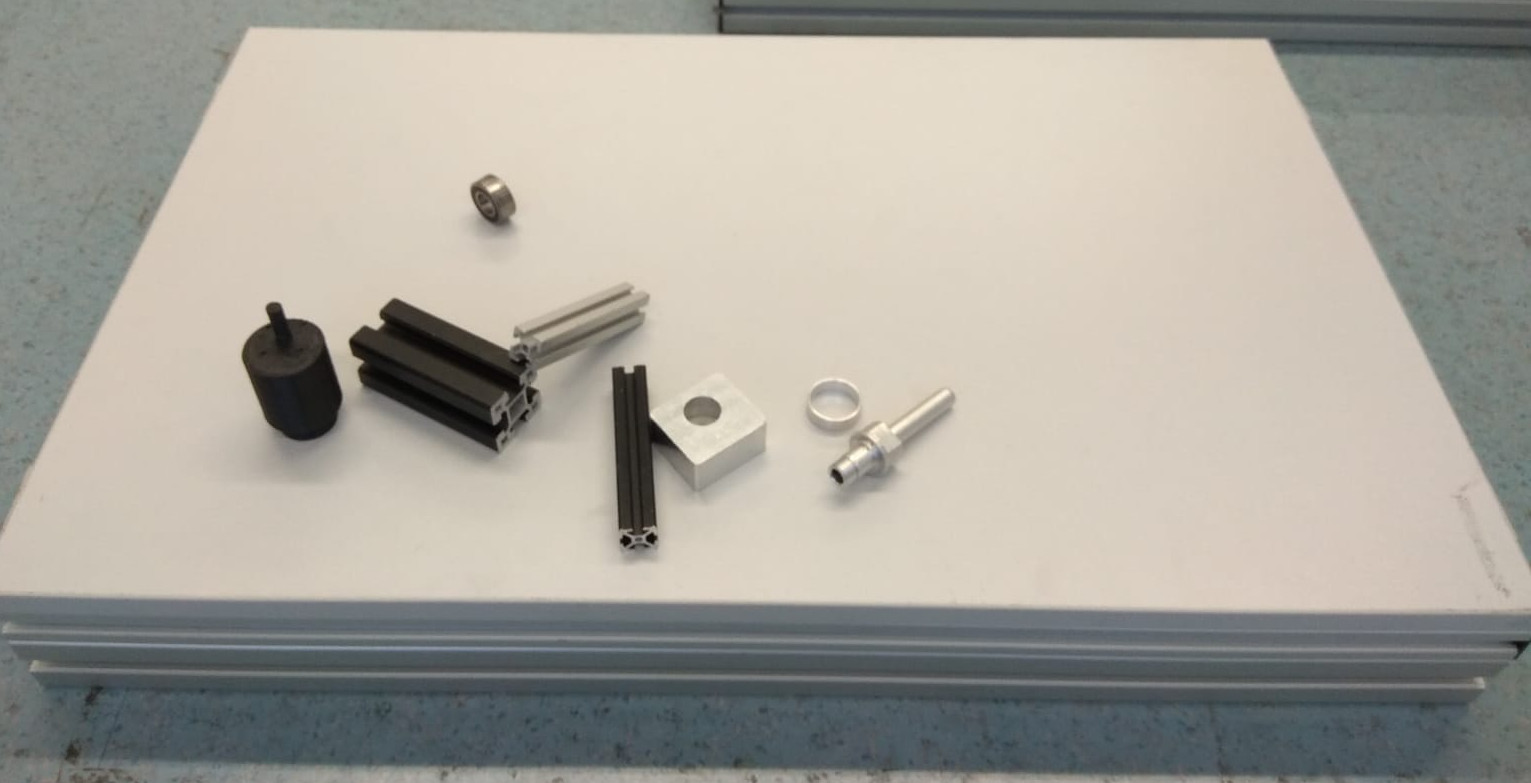
\includegraphics[height = 3cm]{./images/cluttered_pick_1.jpg}} \hspace{1cm}
\subfloat[]{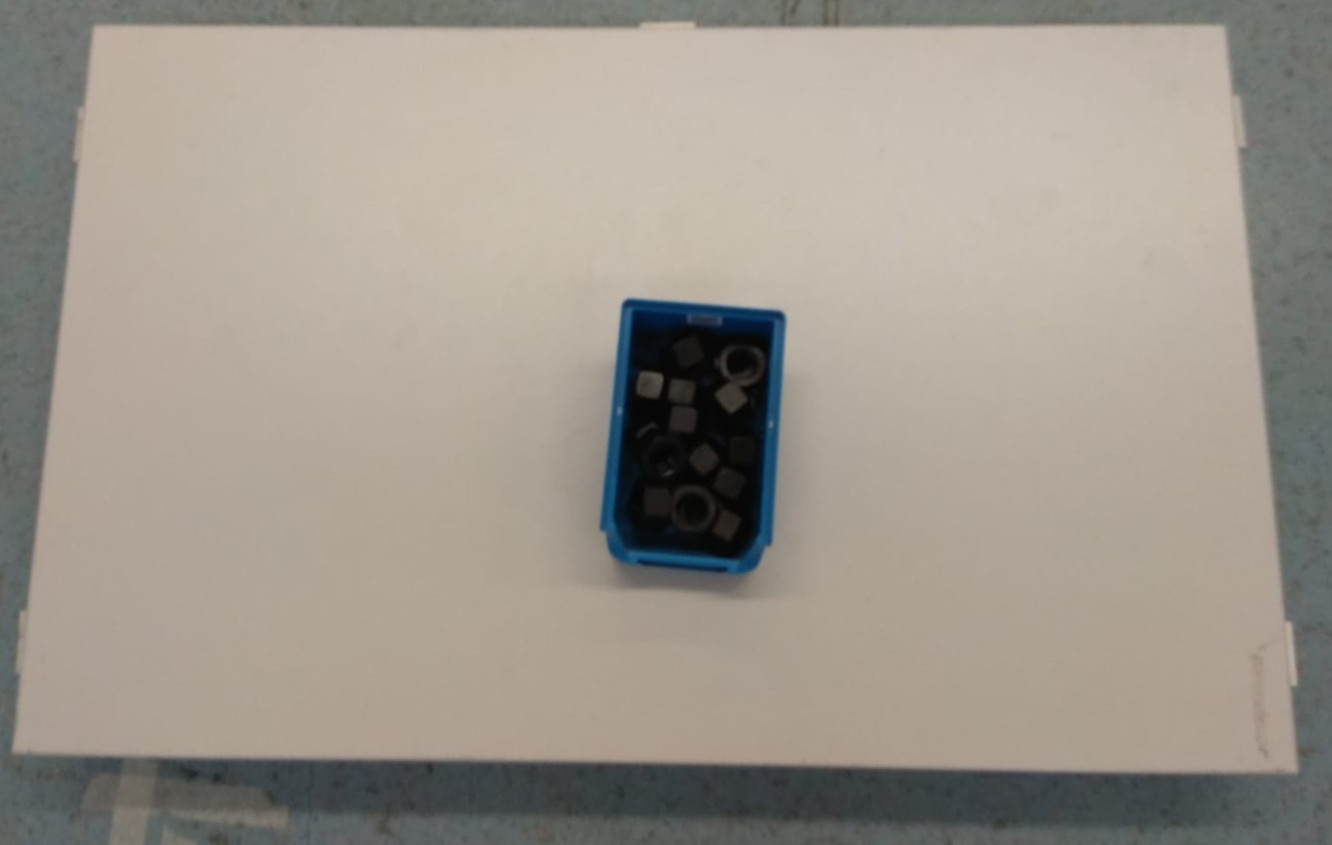
\includegraphics[height = 3cm]{./images/cluttered_pick_2.jpg}}
\end{center}
\caption{objects places in cluttered environment}
\label{fig:clutter}
\end{figure}


\subsection{Variation}
A slight variation in the competition will be to run with 2 robots simultaneously competing with each other.
For fairness of the competition the organizers should ensure that the distance between the robot starting 
point and the corresponding service station be equal.
 
\subsection{Task}
The robot starts at the defined start position outside the arena.
The task consists of navigating to the specified service area containing all the 
requested object. The robot localizes and identifies the object and picks.
The task consists of a sequence of grasp operations. The objective is to pick up all 3 instance of the requested type and avoid picking other objects.
\par
The task specification consists of:
\begin{itemize}
	\item[--] The specification of the initial place
	\item[--] A source location, given as place (e.g. \texttt{WS09})
	\item[--] A list of objects to be manipulated from the source location.
	\item[--] The specification of a final place for the robot
\end{itemize}

\paragraph{Manipulation Objects}
The manipulation objects used in this test are defined by the instances described in Table~\ref{tab:Instances}.

\subsection{Rules}
The following rules have to be obeyed:

\begin{itemize}
\item A single robot is used.
\item The robot has to start from outside the arena and to end in the final.
\item The order in which the teams have to perform will be determined by a draw.
\item At the beginning of a team's period, the team will get the task specification.
\item A service area counts as successfully reached as defined in Section~\ref{ssec:Navigating}
\item Three objects have to be picked.
\item There will be 3-5 decoy objects that must not be picked on the service area.
\item A manipulation object counts as successfully grasped as specified in Section~\ref{ssec:GraspingObjects}.
\item The run is over when the robot reached the final place or the designated time has expired.
\end{itemize}

\subsection{Scoring}
\begin{itemize}
\item 100 points are awarded for each correctly and successfully picked object
\item -50 points for every incorrectly picked object
\item 25 points for reaching the correct service area
\item 25 points for reaching the final position
\end{itemize}
